\chapter{Captura XADC y memoria FIFO}
\label{section:xadc_fifo}


Como se ha introducido anteriormente, en este capítulo se definirá el proceso de captura y conversión de una señal de entrada triangular y el posterior almacenamiento de la misma en una memoria FIFO. En la Figura \ref{fig:xadc_fifo} se muestra el diseño de los bloques necesarios para esta fase y la definición de sus correspondientes puertos de entrada y salida.

\vspace{3mm}

    \begin{figure}[h]
    	\centering
    	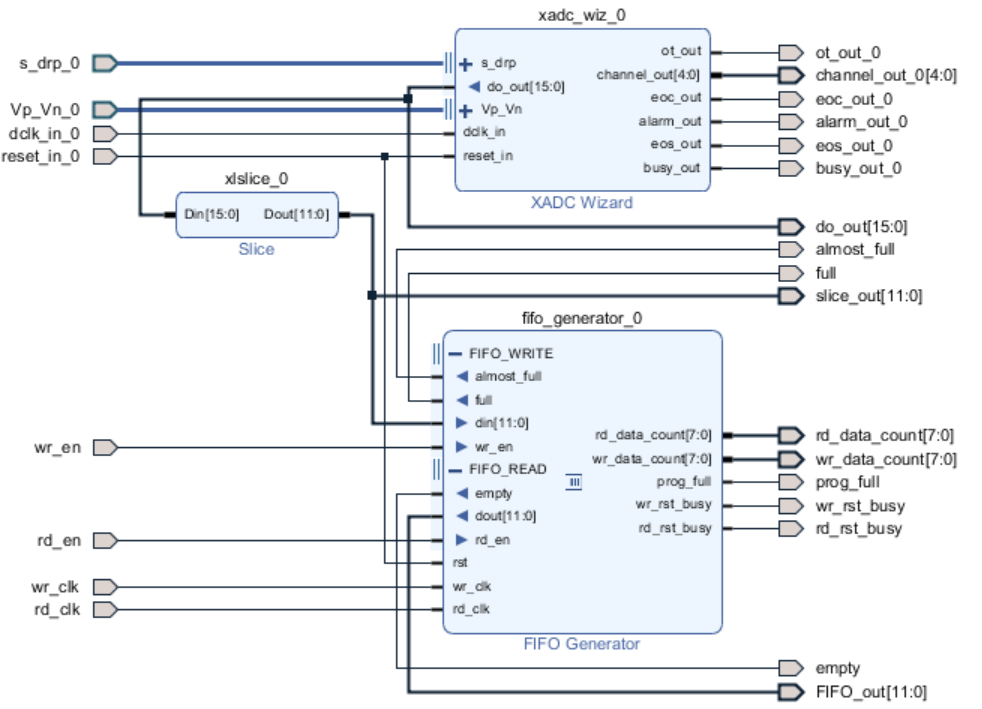
\includegraphics[width=1\textwidth]{img/diseno/xadc_fifo.PNG}
    	\caption{Diseño del bloque XADC+FIFO}
    	\label{fig:xadc_fifo}
    \end{figure}
    
\vspace{3mm}

\section{Obtención de los datos convertidos del ADC}

\subsection{Configuración del XADC}

En primer lugar, teniendo en cuenta que nuestro puesto de laboratorio es el 8, se debe generar a la entrada una señal triangular con un valor de frecuencia igual a 13KHz y que opere en un rango de valores de tensión entre 0 y 0.596 voltios. Los valores que toma en cada instante temporal serán definidos en el fichero design.txt, el cual tendrá que ser importado al proyecto para llevar a cabo la conversión.

Como se puede ver en la Figura \ref*{fig:design} se definen valores de tensión para dos entradas (VP y VN), que corresponden a las entradas analógicas diferenciales del XADC. Por simplificación, se configura el valor absoluto de tensión para la entrada positiva (VP) y un valor nulo para la negativa (VN). 

\vspace{3mm}

    \begin{figure}[h]
    	\centering
    	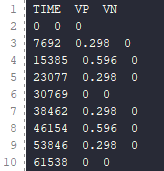
\includegraphics[width=0.3\textwidth]{img/diseno/design.PNG}
    	\caption{Valores de tensión (V) de la señal triangular extraídos de design.txt}
    	\label{fig:design}
    \end{figure}
    
\vspace{3mm}

%el escalon max del ADC = (3/4096)/2 -> el error max, la precisión tiene que ser menor que el error, si no se pierde resolución.
%en vp_vn se pone una precisión segun esto
%0.000366 -> precisión de 10e-4, tensiones de 4 decimales.

El XADC se configura en modo continuo y con un único canal de entrada para capturar las muestras, por lo que se ha seleccionado el canal 3 para registrar el valor convertido de tensión (\textit{s\_drp\_daddr}). La conversión se realizará a una velocidad de 1 MS/seg con un reloj de 52 MHz y se establecerá un tiempo de adquisición igual a 4 para que la señal de captura sea estable.

%hablar de la configuración del xadc
%poner foto del esquema de la documentación
%hablar del 192mhz



\subsection{Simulación de la señal de entrada}

Una vez configurado el bloque IP XADC se procede a simular la conversión de la señal de entrada. En la figura \ref{fig:xadc} se puede visualizar cómo se obtiene la salida digital de 16 bits por el puerto \textit{do\_out}.

\vspace{3mm}

\begin{figure}[h]
    \centering
    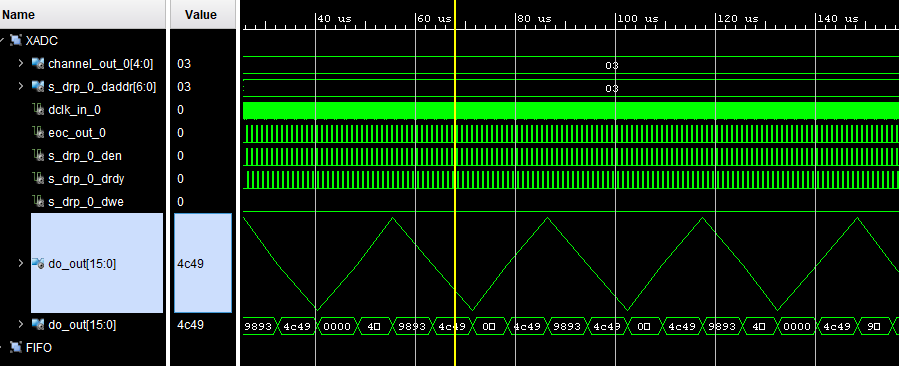
\includegraphics[width=1\textwidth]{img/simu/xadc.PNG}
    \caption{Conversión analógico-digital de la señal triangular de entrada (I)}
    \label{fig:xadc}
\end{figure}

\vspace{3mm}

Por otro lado, en la Figura \ref{fig:xadc2} se aprecia de una forma más clara los valores que toman cada uno de los puertos del XADC en cada conversión. La señal de fin de conversión \textit{eoc\_out} se activa y como consecuencia, también lo hará la de enable del Puerto de Reconfiguración Dinámico (DRP) \textit{eoc\_out}. La operación de lectura se completa cuando la señal de dato ready se activa \textit{s\_drp\_drdy}, indicando que se ha sacado el dato a la salida y que se puede proceder a convertir el siguiente.

\vspace{3mm}

\begin{figure}[h]
    \centering
    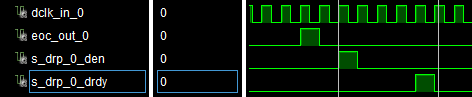
\includegraphics[width=0.7\textwidth]{img/simu/xadc2.PNG}
    \caption{Fin de conversión y dato preparado (III)}
    \label{fig:xadc2}
\end{figure}

\vspace{3mm}

\section{Lógica de control de lectura y escritura de los datos de la FIFO}

\subsection{Configuración del bloque FIFO}

El bloque de memoria FIFO almacenará cada uno de los datos capturados por el bloque XADC. Consta de una capacidad de 256 posiciones de 12 bits cada una, por lo que a la entrada del bloque FIFO será precisa la configuración de un bloque auxiliar Slice para transformar los 16 bits de la señal de salida del XADC en sus 12 bits de mayor peso. Además, esto es necesario porque el XADC en el fondo maneja una precisión de 12 bits a la salida. 

Cada vez que exista un nuevo dato proporcionado por el XADC se escribirá en la memoria FIFO de forma continua a 1 MS/s y con un reloj de 52 MHz (\textit{wr\_clk}) hasta llegar a la capacidad máxima. Una vez la memoria FIFO está llena, comenzará el proceso de lectura de 200 datos a una frecuencia de lectura de 2MHz (\textit{rd\_clk}). En este caso, al desear leer un número de datos menor a la capacidad máxima (256), será necesario configurar una señal auxiliar programable (\textit{programable\_full}).

\vspace{3mm}

    \begin{figure}[h]
    	\centering
    	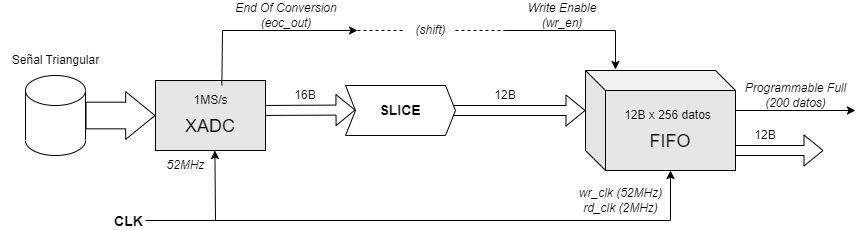
\includegraphics[width=1\textwidth]{img/diseno/xadc_fifo.drawio.PNG}
    	\caption{Diseño del bloque XADC+FIFO}
    	\label{fig:xadc_fifo}
    \end{figure}
    
\vspace{3mm}

\subsection{Comprobación del bloque FIFO}

%explicar como esta relacionado con el xadc
%configuración de contadores de lectura y escritura
      
       % for i in 0 to 200 -- a la espera de 200 datos 
        %loop     
        %    dato_i <= i;